\documentclass{article}
\usepackage[utf8]{inputenc}
\usepackage{graphicx}
\usepackage{float}
\usepackage{hyperref}
\usepackage{listings}
\usepackage{xcolor}

\definecolor{codegreen}{rgb}{0,0.6,0}
\definecolor{codegray}{rgb}{0.5,0.5,0.5}
\definecolor{codepurple}{rgb}{0.58,0,0.82}
\definecolor{backcolour}{rgb}{0.95,0.95,0.92}

\lstdefinestyle{mystyle}{
    backgroundcolor=\color{backcolour},   
    commentstyle=\color{codegreen},
    keywordstyle=\color{magenta},
    numberstyle=\tiny\color{codegray},
    stringstyle=\color{codepurple},
    basicstyle=\ttfamily\footnotesize,
    breakatwhitespace=false,         
    breaklines=true,                 
    captionpos=b,                    
    keepspaces=true,                 
    numbers=left,                    
    numbersep=5pt,                  
    showspaces=false,                
    showstringspaces=false,
    showtabs=false,                  
    tabsize=2
}

\lstset{style=mystyle}

\title{CMS/CS/EE 144 - Homework 1 Analysis Report}
\author{}
\date{}

\begin{document}

\maketitle

\section*{AI Use Declaration}
I manually implemented the initial version of the crawler. I used AI assistance to optimize the crawler by parallelizing it across 5 workers and to help visualize the network structure. For the analysis, I used AI to identify the correct NetworkX functions for calculating diameter and clustering coefficients, as well as to clean histograms and CCDFs. Finally, AI was used to help format this \LaTeX\ report.

\section*{1.1.1 Code \& Execution}

\textbf{Libraries:} The crawler uses \texttt{networkx} for graph management, \texttt{matplotlib} for plotting, and \texttt{concurrent.futures} for parallel execution.

\textbf{How to run:}
\begin{enumerate}
    \item Run the crawler: \texttt{python crawler.py} \\ This generates the graph, saves it to \texttt{caltech\_web\_graph.pkl}, and creates the network visualization.
    \item Run the analysis: \texttt{python analysis.py} \\ This calculates metrics and generates the histograms/CCDFs.
\end{enumerate}

\lstinputlisting[language=Python, caption=Crawler Implementation]{crawler.py}
\lstinputlisting[language=Python, caption=Analysis Implementation]{analysis.py}

\section*{1.1.2 Selection Policy}

We utilized a \textbf{Breadth-First Search (BFS)} selection policy. The crawler maintains a FIFO (First-In-First-Out) queue of URLs.

\textbf{Strengths:}
\begin{itemize}
    \item \textbf{Trap Avoidance:} BFS is less susceptible to "infinite depth" traps (e.g., infinite calendar next-page links) compared to Depth-First Search (DFS).
    \item \textbf{Relevance:} It prioritizes nodes closer to the root (\textit{caltech.edu}), which are typically more significant than deeply nested pages.
    \item \textbf{Parallelism Friendly:} The level-by-level exploration naturally supports our parallel batch processing approach.
\end{itemize}

\textbf{Weaknesses:}
\begin{itemize}
    \item \textbf{Memory Overhead:} The frontier queue can grow large quickly as it stores all discovered-but-not-visited links.
\end{itemize}

\section*{1.1.3 Network Visualization}

\begin{figure}[H]
    \centering
    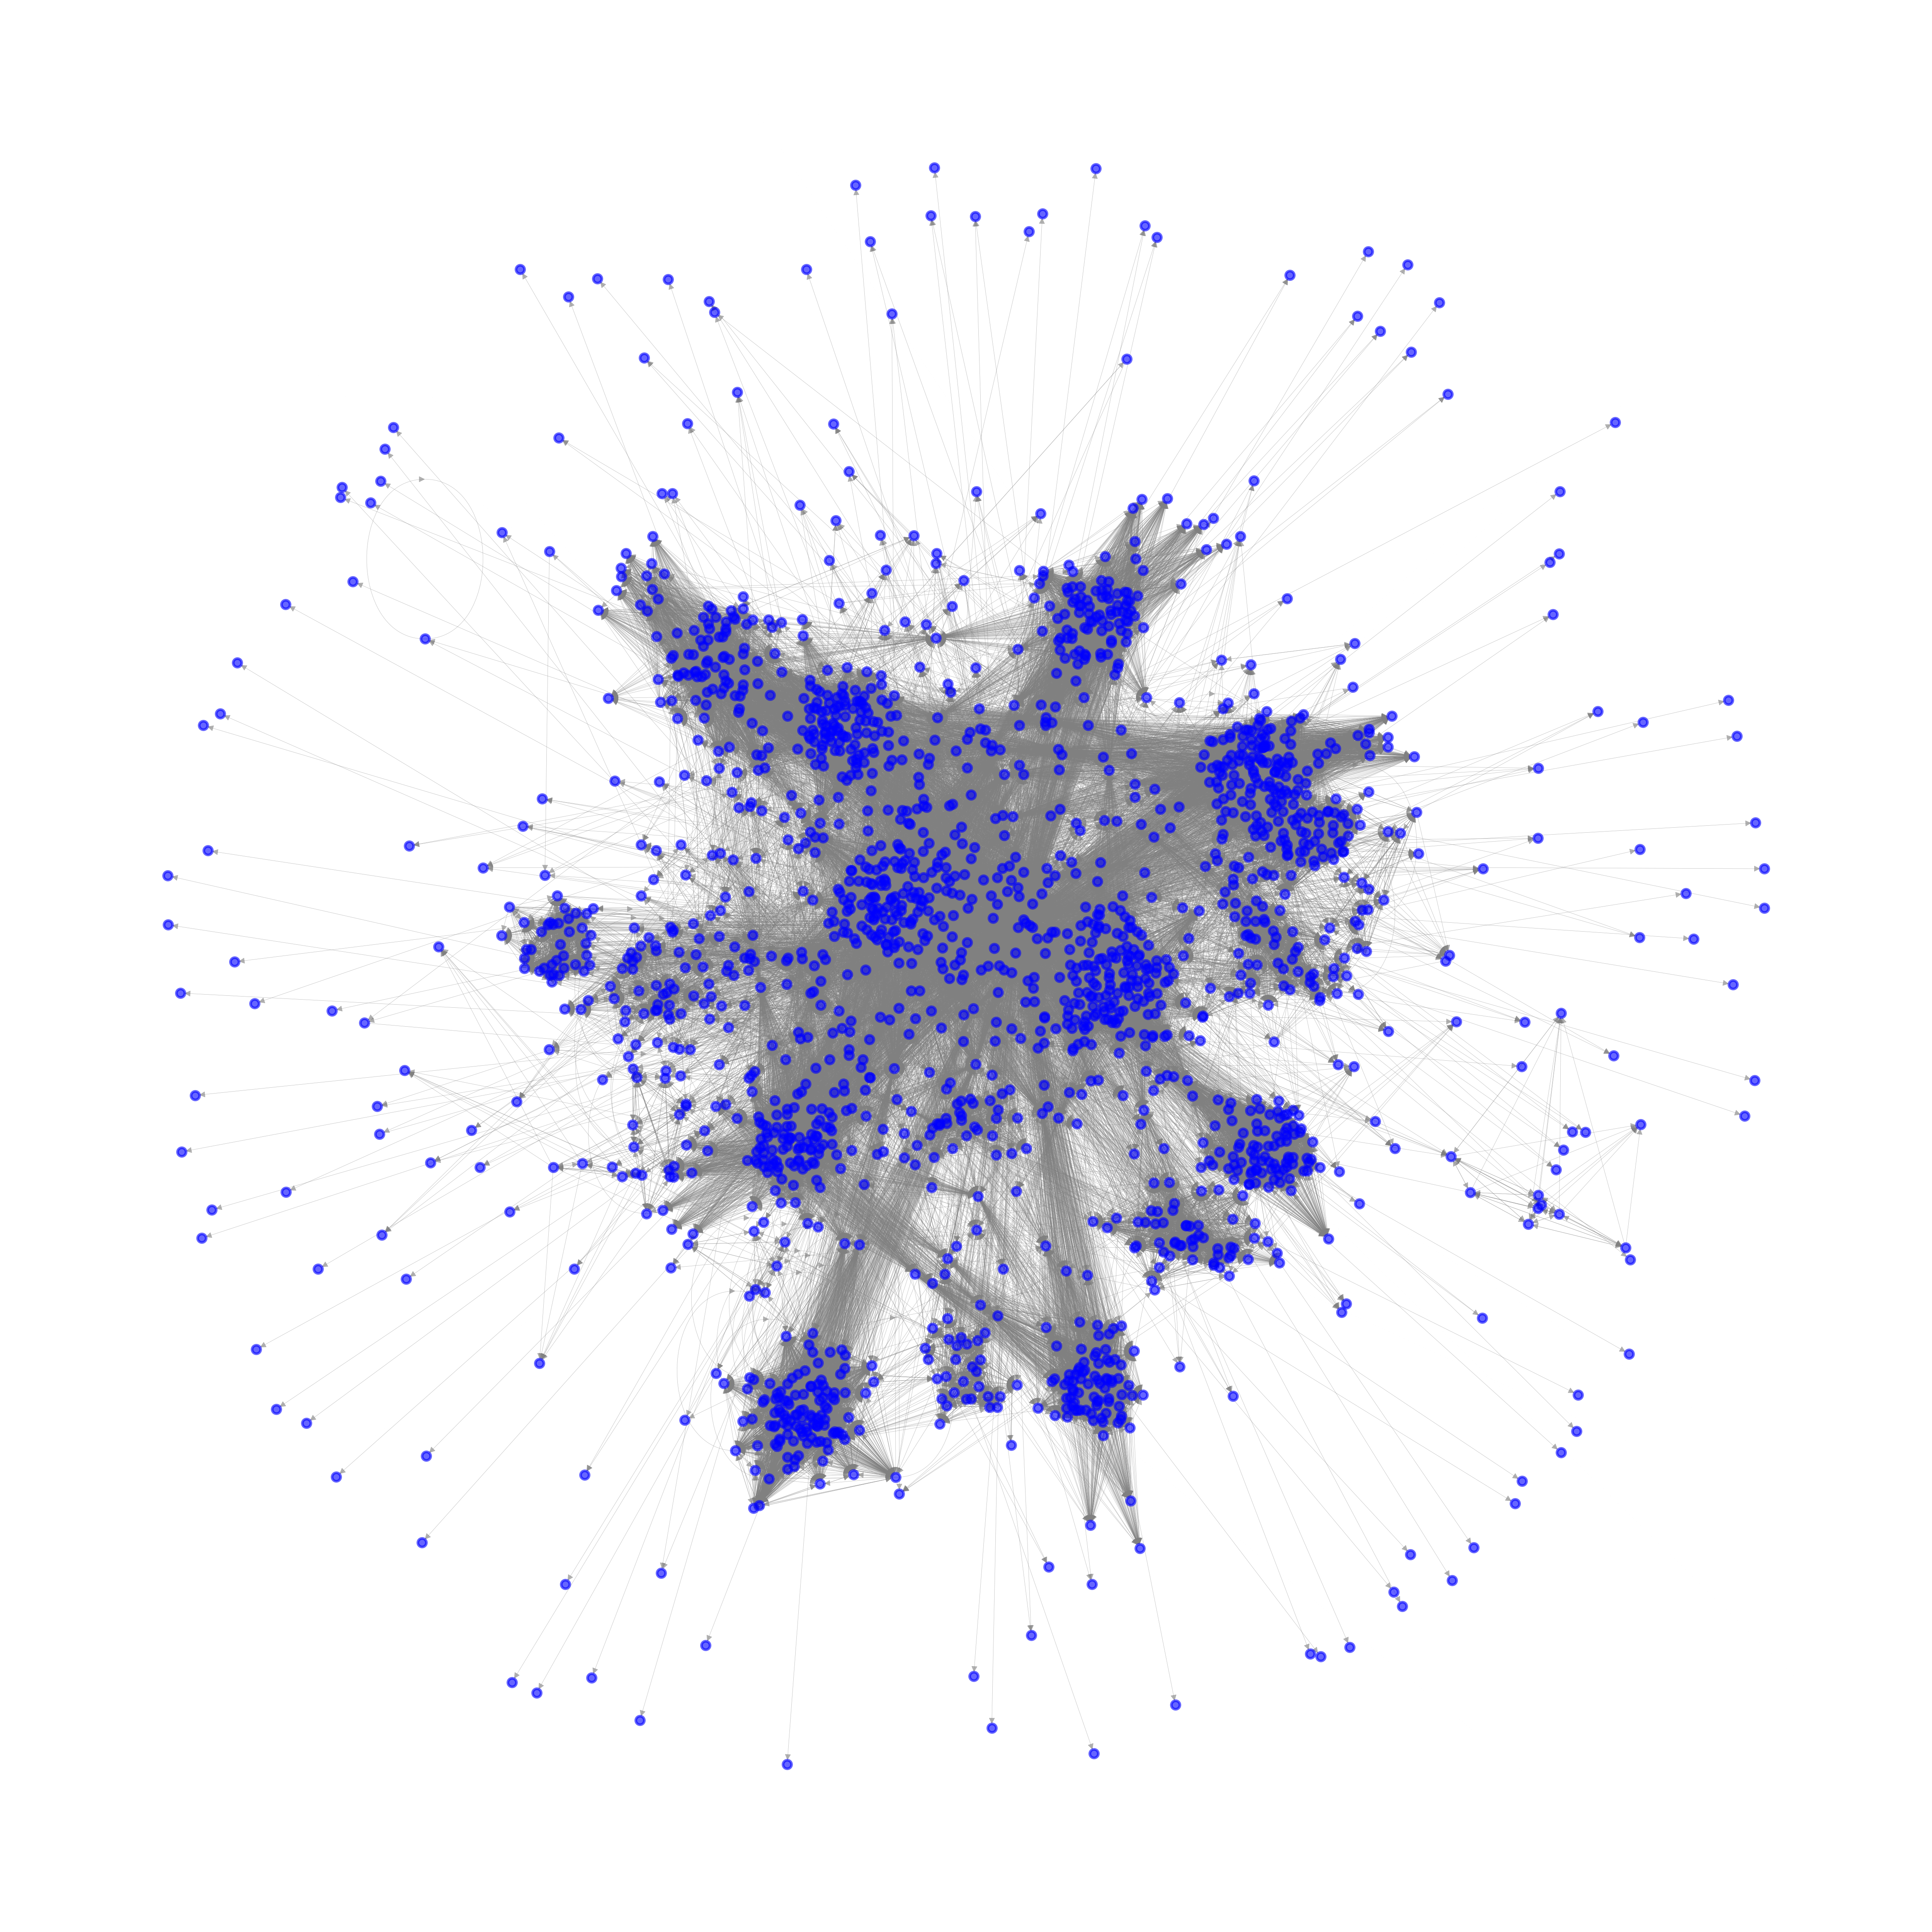
\includegraphics[width=0.9\linewidth]{caltech_web_graph.png}
    \caption{Visualization of the crawled Caltech web graph (Parallel).}
\end{figure}

\section*{1.1.4 Degree Distributions}

\begin{figure}[H]
    \centering
    \begin{minipage}{0.48\textwidth}
        \centering
        \includegraphics[width=\linewidth]{hist_out_degree.png}
        \caption{Out-Degree Histogram}
    \end{minipage}\hfill
    \begin{minipage}{0.48\textwidth}
        \centering
        \includegraphics[width=\linewidth]{ccdf_out_degree.png}
        \caption{Out-Degree CCDF (Log-Log)}
    \end{minipage}
\end{figure}

\begin{figure}[H]
    \centering
    \begin{minipage}{0.48\textwidth}
        \centering
        \includegraphics[width=\linewidth]{hist_in_degree.png}
        \caption{In-Degree Histogram}
    \end{minipage}\hfill
    \begin{minipage}{0.48\textwidth}
        \centering
        \includegraphics[width=\linewidth]{ccdf_in_degree.png}
        \caption{In-Degree CCDF (Log-Log)}
    \end{minipage}
\end{figure}


\section*{1.1.5 Clustering Coefficients}

The following values were calculated treating edges as undirected:

\begin{itemize}
    \item \textbf{Average Clustering Coefficient:} 0.7867
    \item \textbf{Overall Clustering Coefficient:} 0.5905
\end{itemize}


\section*{1.1.6 Diameter Metrics}

Calculated on the largest connected component of the undirected graph:

\begin{itemize}
    \item \textbf{Maximal Diameter:} 4
    \item \textbf{Average Diameter:} 2.4183
\end{itemize}


\section*{1.1.7 Comparison with Collaboration Networks}

\textbf{Task:} A comparison of the degree distribution, the clustering coefficients, and the diameters with those in Problem 2. Can you describe the similarities and differences regarding the "universal" properties between collaboration network and the web graph?

\begin{itemize}
    \item \textbf{Similarities:}
    % TODO: Discuss scale-free nature (power law), small world property (small diameter relative to size).
    
    \item \textbf{Differences:}
    % TODO: Compare specific clustering values (web usually has lower clustering than social/collab networks). Compare exponent of power law if visible.
\end{itemize}

\section*{1.1.8 Sequential Analysis (Retry)}

The Cumulative Distribution Functions (CDFs) from the initial parallel crawl did not exhibit a clear power law behavior, which was unexpected for a web graph. Suspecting that the parallel execution might have influenced the sampling or traversal order non-deterministically, I implemented a sequential version of the crawler to verify the results.

\lstinputlisting[language=Python, caption=Sequential Crawler Implementation]{crawler_NP.py}

\begin{figure}[H]
    \centering
    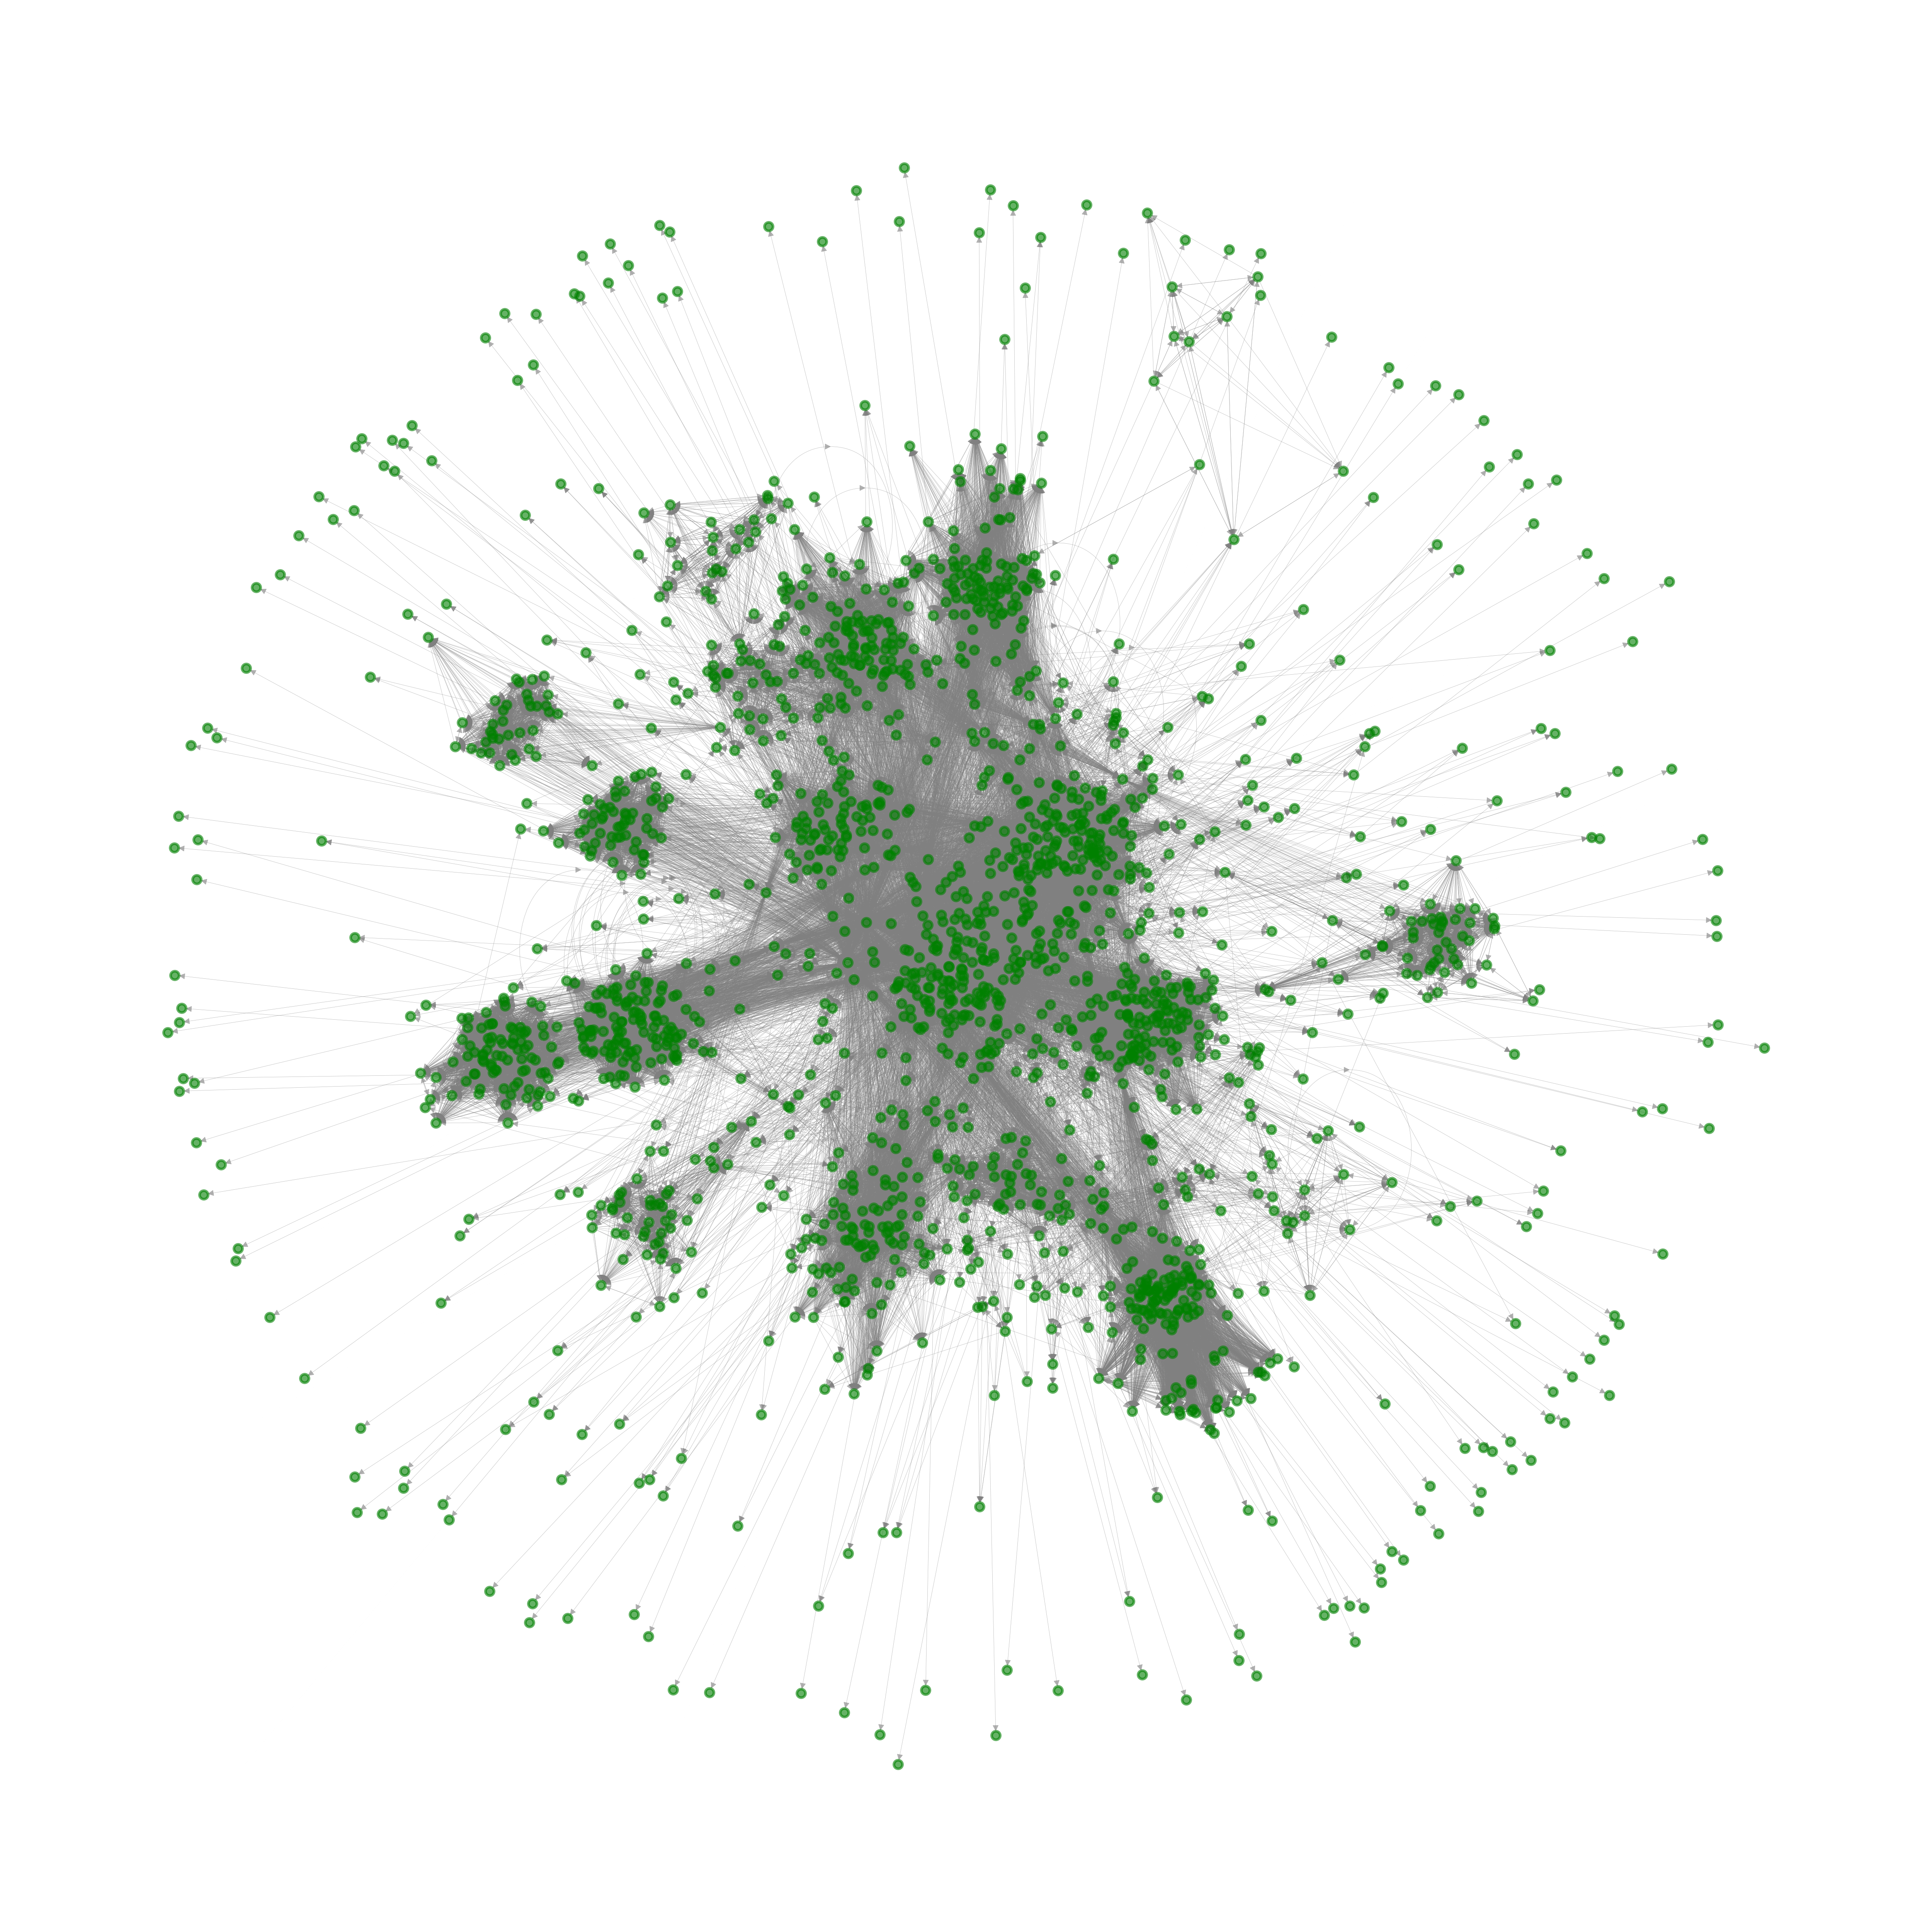
\includegraphics[width=0.9\linewidth]{caltech_web_graph_np.png}
    \caption{Visualization of the Caltech web graph (Sequential).}
\end{figure}

\begin{figure}[H]
    \centering
    \begin{minipage}{0.48\textwidth}
        \centering
        \includegraphics[width=\linewidth]{seq_hist_out_degree.png}
        \caption{Sequential Out-Degree Histogram}
    \end{minipage}\hfill
    \begin{minipage}{0.48\textwidth}
        \centering
        \includegraphics[width=\linewidth]{seq_ccdf_out_degree.png}
        \caption{Sequential Out-Degree CCDF (Log-Log)}
    \end{minipage}
\end{figure}

\begin{figure}[H]
    \centering
    \begin{minipage}{0.48\textwidth}
        \centering
        \includegraphics[width=\linewidth]{seq_hist_in_degree.png}
        \caption{Sequential In-Degree Histogram}
    \end{minipage}\hfill
    \begin{minipage}{0.48\textwidth}
        \centering
        \includegraphics[width=\linewidth]{seq_ccdf_in_degree.png}
        \caption{Sequential In-Degree CCDF (Log-Log)}
    \end{minipage}
\end{figure}

The metrics for the sequential graph are:
\begin{itemize}
    \item \textbf{Average Clustering Coefficient:} 0.7526
    \item \textbf{Overall Clustering Coefficient:} 0.6106
    \item \textbf{Maximal Diameter:} 4
    \item \textbf{Average Diameter:} 2.5954
\end{itemize}

\textbf{Conclusion:} The results from the sequential crawler are very similar to the parallel version. The graph structure, degree distributions, and clustering coefficients show no significant differences, suggesting that the parallel implementation correctly captures the graph properties and the observed distributions are intrinsic to the crawled subgraph.


\section*{1.2(a) Flight to the Queen Bee}

The following paths were discovered on \href{https://www.music-map.com/}{music-map.com}. In both instances, the first path found was also the shortest.

\begin{itemize}
    \item \textbf{Nikolai Rimsky-Korsakov $\rightarrow$ Beyoncé} \\
    Path: Nikolai Rimsky-Korsakov $\rightarrow$ Mozart $\rightarrow$ Distant Fires Burning $\rightarrow$ Chanyeol $\rightarrow$ BTS $\rightarrow$ Arctic Monkeys $\rightarrow$ Ed Sheeran $\rightarrow$ Adele $\rightarrow$ Beyoncé

    \item \textbf{Lyle Mays $\rightarrow$ Taylor Swift} \\
    Path: Lyle Mays $\rightarrow$ John Taylor $\rightarrow$ Mick Fleetwood $\rightarrow$ U2 $\rightarrow$ The Beatles $\rightarrow$ One Direction $\rightarrow$ Olivia Rodrigo $\rightarrow$ Taylor Swift
\end{itemize}

\section*{1.2(b) Know your Professors}

The following paths were found using the ``Co-authorship Path'' tool on \href{https://csauthors.net}{csauthors.net}.

\begin{enumerate}
    \item \textbf{Eric Mazumdar $\rightarrow$ Rudolf E. K\'alm\'an} (Distance: 5) \\
    Source: \href{https://csauthors.net/distance/eric-mazumdar/rudolf-e-kalman}{https://csauthors.net/distance/eric-mazumdar/rudolf-e-kalman}
    \begin{itemize}
        \item Eric Mazumdar co-authored \textbf{10 papers} with Adam Wierman
        \item Adam Wierman co-authored \textbf{8 papers} with Linqi Guo
        \item Linqi Guo co-authored \textbf{4 papers} with Guangyi Shi
        \item Guangyi Shi co-authored \textbf{1 paper} with Kazuo Toraichi
        \item Kazuo Toraichi co-authored \textbf{2 papers} with Rudolf E. K\'alm\'an
    \end{itemize}

    \item \textbf{Georgia Gkioxari $\rightarrow$ Paul Erd\H{o}s} (Distance: 3) \\
    Source: \href{https://csauthors.net/distance/georgia-gkioxari/paul-erdos}{https://csauthors.net/distance/georgia-gkioxari/paul-erdos}
    \begin{itemize}
        \item Georgia Gkioxari co-authored \textbf{12 papers} with Jitendra Malik
        \item Jitendra Malik co-authored \textbf{2 papers} with Fan Chung Graham
        \item Fan Chung Graham co-authored \textbf{7 papers} with Paul Erd\H{o}s
    \end{itemize}
\end{enumerate}

\section*{1.2(d) Citations}

I attempted to find paths for this section for over 30 minutes using multiple tools, including \textit{Inciteful} and large language models like \textit{Gemini}.

\begin{itemize}
    \item \textbf{Inciteful:} This tool was problematic because it did not strictly follow the directed edge requirement (A cites B). Instead, it often connected papers if they simply cited the same source, resulting in invalid paths for this specific task. It found a distance of 3, but this was based on undirectional logic.
    \item \textbf{Gemini / LLMs:} Gemini proposed paths such as \textit{Zipf (1936)} $\rightarrow$ \textit{Simon (1955)} $\rightarrow$ \textit{Price (1965)} $\rightarrow$ \textit{Granovetter (1973)} and \textit{Kalman (1960)} $\rightarrow$ \textit{Bryson \& Ho (1969)} $\rightarrow$ \textit{Rumelhart et al. (1986)} $\rightarrow$ \textit{LeCun et al. (1998)}. However, verifying these specific citation links manually was extremely difficult and time-consuming, as it required accessing the full text of each paper to confirm the bibliography entries.
\end{itemize}

Due to these difficulties and the unreliability of automated tools for strict directed citation verification, I was unable to definitively confirm a valid path.

\end{document}
